\section{Results}
\begin{frame}
\frametitle{Numerical Setup} 
\begin{block}{A square periodic domain}
 \begin{itemize}
  \item Total number of particles: $512 \times 512 = 262144$.
  \item Domain size: $ 0.0128\times 0.0128$.
  \item Polymer chains: $8$ beads and $16$ beads.
 \end{itemize}
\begin{table}
\begin{center}
  \begin{tabular}{| c | c | c |  c| c | c | c | c | c |}
    \hline
    Parameter & $\Delta x$ & $\rho$ & c & $\eta$ & $K$ & $R_0$ & $\delta$ \\ 
    \hline
    Value & $2.5E-5$ & 1 & 10 & 0.003 & 0.01 & 4.0 & 1.0 \\ 
   \hline
  \end{tabular}
\end{center}
\caption {The value of parameters in simulation}
\label{tab:roll}
\end{table}
\end{block}



\end{frame}


\begin{frame}
  \frametitle{Flow of Pure Solvent}
%   \begin{itemize}
%   \item Initial condition: ``seed'' vapor particles in the center of
%     the domain
%   \item Domain is periodic, edges of the domain $T=T_s +
%     \Delta T$
%   \item Theory predicts a self similar temperature profile $T =
%     T(r/R(t))$, where $r$~---~distance from the center, $R(t)$~---~radius of
%     the bubble
%   \end{itemize}

\begin{figure}
    \centering
    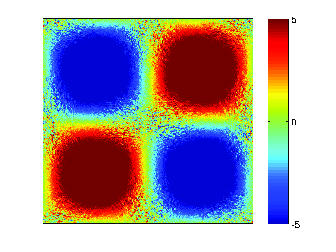
\includegraphics[width=0.5\textwidth]{img/polymer_loc-15.png}
    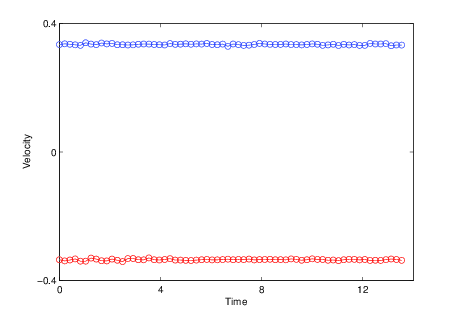
\includegraphics[width=0.5\textwidth]{img/polymer_loc-9.png}
    \caption{Vorticity field and velocity of one point $P_0=[5/8L,5/8L]$ in flow of pure solvent flow at $Re\approx 80$.}
    \label{fig:vor_sol}
  \end{figure}
\end{frame}

\begin{frame}
  \frametitle{Flow of Polymer Solution}
  \begin{figure}
    \centering
    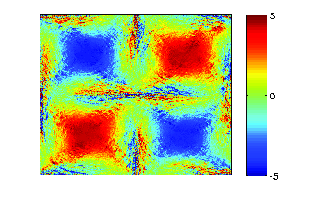
\includegraphics[width=0.6\textwidth]{img/polymer_loc-10.png}
  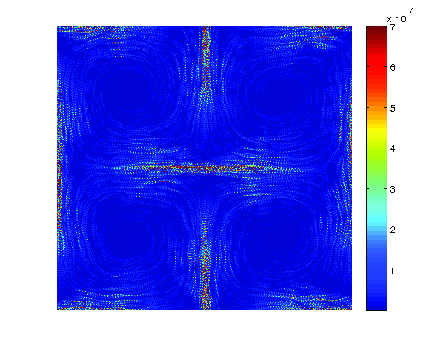
\includegraphics[width=0.5\textwidth]{img/polymer_loc-6.png}
    \caption{Vorticity field and elastic stress trace in flow of polymer solution at $Wi\approx1$.}
    \label{fig:vor_pol1}
  \end{figure}
\end{frame}

\begin{frame}
  \frametitle{Flow of Polymer Solution}
\begin{figure}[ht]
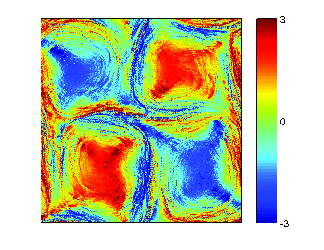
\includegraphics[width=0.5\textwidth]{img/polymer_loc-13.png}
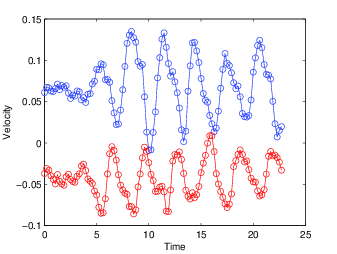
\includegraphics[width=0.5\textwidth]{img/polymer_loc-7.png}
\caption{Vorticity field and velocity of the point $P_0$ in flow of polymer solution at $Wi\approx5$.}
\label{fug:vor_pol5}
\end{figure}
\end{frame}
% \begin{frame}
%   \frametitle{Flow of Polymer Solution}
%   \begin{figure}[ht]
% 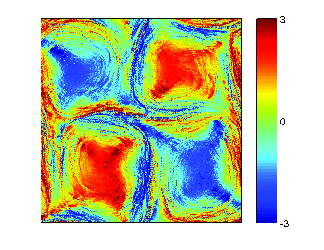
\includegraphics[width=0.5\textwidth]{img/polymer_loc-13.png}
% 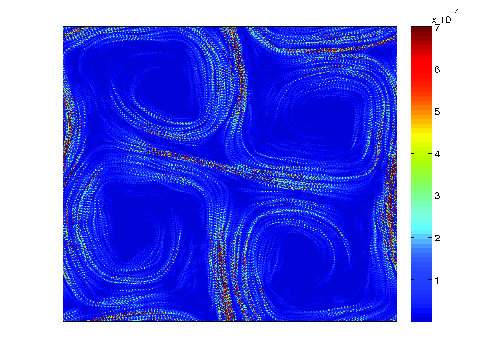
\includegraphics[width=0.5\textwidth]{img/polymer_loc-5.png}
% \caption{Velocity and elastic stress trace in flow of polymer solution at $Wi\approx5$.}
% \label{fug:vel_pol5}
% \end{figure}
% \end{frame}

\begin{frame}
 \begin{figure}
    \centering
    \includegraphics[width=0.51\textwidth]{img/polymer_global.jpg}
    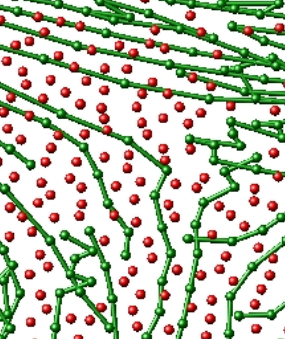
\includegraphics[width=0.4\textwidth]{img/polymer_local_3}

    \caption{Snapshot of polymer solution at $Wi\approx5$ in global and local view,respectively.}
    \label{fig:vor_sol}
  \end{figure}
\end{frame}

\begin{frame}
  \frametitle{Flow of Polymer Solution}
  \begin{figure}[ht]
    \centering
    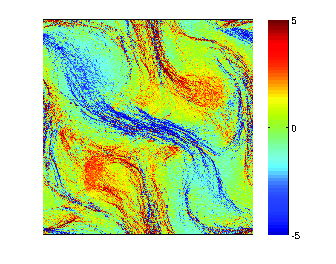
\includegraphics[width=0.5\textwidth]{img/polymer_loc-14.png}
    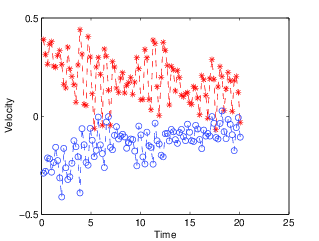
\includegraphics[width=0.5\textwidth]{img/polymer_loc-8.png}
    \caption{Vorticity field and velocity of the point $P_0$ in flow of polymer solution at $Wi\approx10$.}
    \label{fig:vor_pol10}
  \end{figure}
\end{frame}

\begin{frame}
 \frametitle{Flow of Polymer Solution}
  \begin{figure}[t]
    \centering
    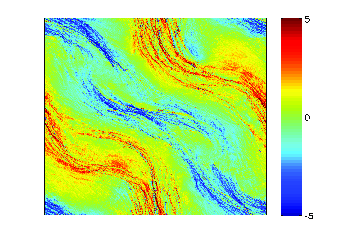
\includegraphics[width=0.5\textwidth]{img/polymer_loc-11.png}
 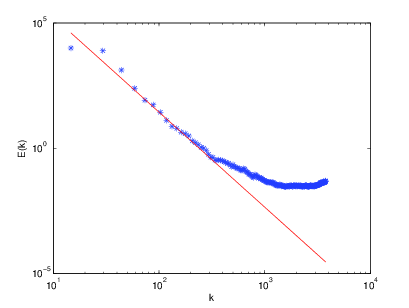
\includegraphics[width=0.5\textwidth]{img/polymer_loc-0.png}
    \caption{Vorticity field and energy spectrum ($E_k\sim k^{-3.8}$) in flow of polymer solution at $Wi\approx10$ with perturbation.}
    \label{fig:vor_per}
  \end{figure}
\bibliographystyle{elsart-num}
\nobibliography{bibdata}
\end{frame}

%%% Local Variables: 
%%% mode: latex
%%% TeX-master: t
%%% End: 
